\documentclass[12pt, legalpaper]{exam}
\usepackage[paper=letterpaper,margin=2cm]{geometry}
\usepackage{amsmath}
\usepackage{amssymb}
\usepackage{amsfonts}
\usepackage{newtxtext, newtxmath}
\usepackage{enumitem}
\usepackage{titling}
\usepackage{listings}
\usepackage{array}
\usepackage{tabularray}
\usepackage[ddmmyyyy]{datetime}
\usepackage{xcolor}
\usepackage{graphicx}
\usepackage{float}
\graphicxpath{  }
\NewColumnType{M}[1]{Q[m,c,#1]}
% \usepackage[colorlinks=false]{hyperref}

% Nastavení hlavičky
\newcommand{\class}{Control Theory}
\newcommand{\term}{Fall semester, 2023}
\newcommand{\examnum}{2}

% Nastavení tabulky bodů
\pointpoints{pt.}{pts.}
\hpword{Max. pts.:}
\hsword{Recieved:}
\hqword{Question:}
\htword{Total:}

\pagestyle{head}
\firstpageheader{University of Chemistry and Technology \\ in Prague}{}{Department of Mathematics, \\ Informatics and Cybernetics}
\runningheader{\class}{Page \thepage\ / \numpages}{Assignment \#\examnum}
\runningheadrule

\begin{document}
\noindent
\begin{tabular*}{\textwidth}{l @{\extracolsep{\fill}} r @{\extracolsep{6pt}} l}
\textbf{\class} & \textbf{Name:} & \makebox[2.5in][l]{ Flore Tiesen }\\
\textbf{Assignment \#\examnum} & \textbf{Date:} & \makebox[2.5in][l]{\today}\\
\end{tabular*}\\

\rule[2ex]{\textwidth}{2pt}

\begin{questions}

        \question Find a transfer function of the second-order system $G(s)$ that has undamped oscillations and oscillates with
        a frequency of $f=9 Hz$. Note that $\omega = 2\pi f$. In Simulink, check that the response of 
	this transfer function to the unit step meets the requirements.

        \question Determine the transfer function $\frac{Y(s)}{U(s)}$ of the following block diagram.
        \begin{figure}[H]
            \centering
            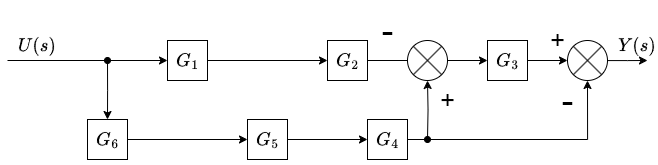
\includegraphics[scale=0.6]{./templates/images/block_18.png}

        \end{figure}

        \question Determine the time delay of the following transfer function:

        \begin{equation*}
            G(s) =  e^{- 1.9 s} \frac{ 3 }{s + 13 }
        \end{equation*}

        Approximate the behavior of the time delay with the second-order Padé approximation.

        \question Using both manual and Ziegler-Nichols tuning methods, set up a PID controller that would control
        a plant with the following transfer function.

        \begin{equation*}
            G(s) =  \frac{1}{s^3 + 2.65s^2 + 4.11s + 2.74}
        \end{equation*}

        Show the resulting control loops in the Simulink environment.

\end{questions}
\end{document}